\chapter{推荐算法概述以及大数据相关技术}

\section{推荐算法概述}
在一个电商系统中,有商品、类目、品牌、团购、闪购、搜索、店铺、广告、促销活动、抵用券等诸多实体;有首页的大轮播、猜你喜欢栏位,详情页的看了还看、看了还买、推荐品牌等栏位,购物车页面的买了还买、凑单免邮等栏位。如何在不同的栏位融入不同的推荐算法给用户推荐相应的实体,构建出属于电商自己的推荐系统,实现全站精准化,让网站的GMV或者利润达到最高,是每一个电商需要思考的问题。
推荐系统并不是新鲜的事物,在很久之前就存在,但是推荐系统真正进入人们的视野,并且作为一个重要的模块存在于各个互联网公司,还是近几年的事情。随着互联网的深入发展,越来越多的信息在互联网上传播,产生了严重的信息过载。如果不采用一定的手段,用户很难从如此多的信息流中找到对自己有价值的信息。
解决信息过载有几种手段:一种是搜索,当用户有了明确的信息需求意图后,将意图转换为几个简短的词或者短语的组合(即query),然后将这些词或短语组合提交到相应的搜索引擎,再由搜索引擎在海量的信息库中检索出与query相关的信息返回给用户;另外一种是推荐,很多时候用户的意图并不是很明确,或者很难用清晰的语义表达,有时甚至连用户自己都不清楚自己的需求,这种情况下搜索就显得捉襟见肘了。尤其是近些年来,随着电子商务的兴起,用户并非一定是带着明确的购买意图去浏览,很多时候是去“逛”的,这种情景下解决信息过载,理解用户意图,为用户推送个性化的结果,推荐系统便是一种比较好的选择。

\begin{figure}[htbp]
\centering 
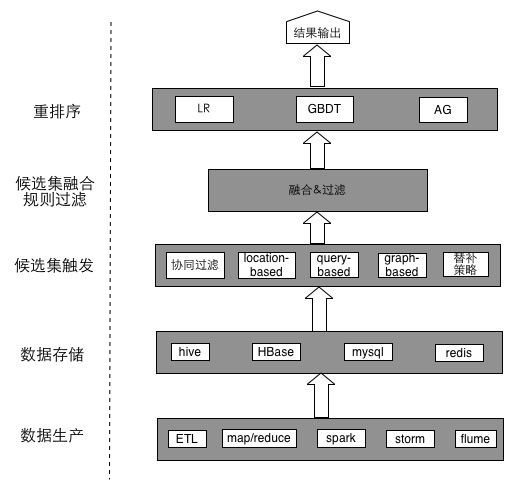
\includegraphics[width=6.5cm]{pic/system_infrastructure.jpg} 
\caption{推荐系统框架图} \label{fig:system_infrastructure} 
\end{figure}
如\ref{fig:system_infrastructure}所示,从框架的角度看,推荐系统基本可以分为数据层、触发层、融合过滤层和排序层。数据层包括数据生成和数据存储,主要是利用各种数据处理工具对原始日志进行清洗,处理成格式化的数据,落地到不同类型的存储系统中,供下游的算法和模型使用。候选集触发层主要是从用户的历史行为、实时行为、地理位置等角度利用各种触发策略产生推荐的候选集。候选集融合和过滤层有两个功能,一是对出发层产生的不同候选集进行融合,提高推荐策略的覆盖度和精度;另外还要承担一定的过滤职责,从产品、运营的角度确定一些人工规则,过滤掉不符合条件的item。排序层主要是利用机器学习的模型对触发层筛选出来的候选集进行重排序。
同时,对与候选集触发和重排序两层而言,为了效果迭代是需要频繁修改的两层,因此需要支持ABtest。为了支持高效率的迭代,我们对候选集触发和重排序两层进行了解耦,这两层的结果是正交的,因此可以分别进行对比试验,不会相互影响。同时在每一层的内部,我们会根据用户将流量划分为多份,支持多个策略同时在线对比。

  \subsection{基于关联规则的推荐}
  基于关联规则的推荐(Association Rule-based Recommendation)是以关联规则为基础,把已购商品作为规则头,规则体为推荐对象。关联规则挖掘可以发现不同商品在销售过程中的相关性,在零 售业中已经得到了成功的应用。管理规则就是在一个交易数据库中统计购买了商品集X的交易中有多大比例的交易同时购买了商品集Y,其直观的意义就是用户在购 买某些商品的时候有多大倾向去购买另外一些商品。比如购买牛奶的同时很多人会同时购买面包。
  算法的第一步关联规则的发现最为关键且最耗时,是算法的瓶颈,但可以离线进行。其次,商品名称的同义性问题也是关联规则的一个难点。

  \subsection{协同过滤}
  协同过滤推荐(Collaborative Filtering Recommendation)技术是推荐系统中应用最早和最为成功的技术之一。它一般采用最近邻技术,利用用户的历史喜好信息计算用户之间的距离,然后利用目标用户的最近邻居用户对商品评价的加权评价值来预测目标用户对特定商品的喜好程度,系统从而根据这一喜好程度来对目标用户进行推荐。协同过滤最大优点是对推荐对象没有特殊的要求,能处理非结构化的复杂对象,如音乐、电影。
  协同过滤是基于这样的假设:为一用户找到他真正感兴趣的内容的好方法是首先找到与此用户有相似兴趣的其他用户,然后将他们感兴趣的内容推荐给此用户。其基本思想非常易于理解,在日常生活中,我们往往会利用好朋友的推荐来进行一些选择。协同过滤正是把这一思想运用到电子商务推荐系统中来,基于其他用户对某一内容的评价来向目标用户进行推荐。
  基于协同过滤的推荐系统可以说是从用户的角度来进行相应推荐的,而且是自动的,即用户获得的推荐是系统从购买模式或浏览行为等隐式获得的,不需要用户努力地找到适合自己兴趣的推荐信息,如填写一些调查表格等。
  User-based 的协同过滤和 Item-based 的协同过滤是两个最常用的技术,它俩统称为Memory based的协同过滤技术,他们共有的缺点是数据稀疏,难以处理大数据量给出即时结果(item-based的协同过滤比user-based的协同过滤稍好一些),因此发展出以模型为基础的协同过滤技术。 以模型为基础的协同过滤(Model-based Collaborative Filtering)是先用历史资料得到一个模型,再用此模型进行预测。以模型为基础的协同过滤广泛使用的技术包括Latent Semantic Indexing、Bayesian Networks等等。
  User-based的协同过滤用相似统计的方法得到具有相似爱好或者兴趣的相邻使用者,以下是它的详细步骤:
  \begin{enumerate}
  \item 收集用户评分,包括主动评分和/或者被动评分。
  \item 最近邻搜索(Nearest neighbor search, NNS):以用户为基础(User-based)的协同过滤的出发点是与用户兴趣爱好相同的另一组用户,就是计算两个用户的相似度。寻找n个和A有相似兴趣用户,然后把他们对M的评分作为A对M的评分预测。
  \item 产生推荐结果
  \end{enumerate}
  有了最近邻集合,就可以对目标用户的兴趣进行预测,产生推荐结果。依据推荐目的的不同进行不同形式的推荐,较常见的推荐算法有Top-N 推荐和关联推荐。Top-N 推荐是针对个体用户产生,对每个人产生不一样的结果,例如:透过对A使用者的最近邻使用者进行统计,选择出现频率高且在A使用者的评分项目中不存在的,作为推荐结果。关联推荐是对最近邻使用者的记录进行关联规则(association rules)挖掘。
  Item-based的协同过滤技术实现方式同 User-based的协同过滤类似,只是分析目标由用户变成了Item。

  \subsection{点击率预估+排序}
  推荐问题可以转化为点击率预估子问题+排序子问题,通过对推荐问题的拆解,原问题转化为对两个子问题建模并最优化求解。因此,需要建立点击率预估模型和排序模型,前者通常使用高纬稀疏特征训练\gls*{LR}模型,而由于LR模型的预测结果是一个正行为的概率,因此LR模型的预测结果天然地可以用于排序,排序子问题可通过TopK排序或阈值方法来解决。除此之外,对于点击率预估子问题还可以使用\gls*{RF}、\gls*{GBDT}等非线性模型,或组合模型来解决。
  子问题相对于原问题,有如下对比:
  \begin{itemize}
  \item 优点
    \begin{itemize}
    \item 单个子模型更容易实现比较准地预估
    \item 可以调整子模型的融合方式,以达到最佳效果
    \end{itemize}
  \item 缺点
    \begin{itemize}
    \item 可能产生积累误差
    \item 训练和应用成本高
    \end{itemize}
  \end{itemize}

    \subsubsection{逻辑回归模型}
    逻辑回归(Logistic Regression)是机器学习中的一种分类模型,由于算法的简单和高效,在实际中应用非常广泛。逻辑回归模型其实仅在线性回归的基础上,套用了一个逻辑函数,但也就由于这个逻辑函数,使得逻辑回归模型成为了机器学习领域一颗耀眼的明星,更是计算广告学的核心。

    \subsubsection{组合模型}
    根据Facebook 2014年的论文《Practical Lessons from Predicting Clicks on Ads at Facebook》\cite{PracticalPredictingFacebook},使用GBDT+LR的组合模型,可以有效地解决LR模型中复杂、耗时且强依赖于领域知识的特征选择问题。Facebook使用GBDT做特征升维,应用在其线上广告系统提高了3\%的指标。

    介绍GBDT blabla


\section{大数据技术概述}

  \subsection{Hadoop}
  Hadoop(http://hadoop.apache.org/)是一个由Apache基金会所开发的分布式系统基础架构。Hadoop是根据Google公司发表的MapReduce和Google文件系统的论文自行实现而成。
  Hadoop框架透明地为应用提供可靠性和数据移动。它实现了名为MapReduce的编程范式:应用程序被分区成许多小部分,而每个部分都能在集群中的任意节点上运行或重新运行。此外,Hadoop还提供了分布式文件系统\gls*{HDFS},用以存储所有计算节点的数据,这为整个集群带来了非常高的带宽。MapReduce和分布式文件系统的设计,使得整个框架能够自动处理节点故障。它使应用程序与成千上万的独立计算的电脑和PB级的数据。现在普遍认为整个Apache Hadoop“平台”包括Hadoop内核、MapReduce、Hadoop分布式文件系统(HDFS)以及一些相关项目,有Apache Hive和Apache HBase等等。
  用户可以在不了解分布式底层细节的情况下,开发分布式程序。充分利用集群的威力进行高速运算和存储。HDFS有高容错性的特点,并且设计用来部署在低廉的(low-cost)硬件上;而且它提供高吞吐量(high throughput)来访问应用程序的数据,适合那些有着超大数据集(large data set)的应用程序。HDFS放宽了POSIX的要求,可以以流的形式访问(streaming access)文件系统中的数据。Hadoop的框架最核心的设计就是:HDFS和MapReduce。HDFS为海量的数据提供了存储框架,则MapReduce为海量的数据提供了计算框架。

    \subsubsection{Hadoop的优点}
    Hadoop是一个能够对大量数据进行分布式处理的软件框架。 Hadoop 以一种可靠、高效、可伸缩的方式进行数据处理。
    Hadoop 是可靠的,因为它假设计算元素和存储会失败,因此它维护多个工作数据副本,确保能够针对失败的节点重新分布处理。Hadoop 是高效的,因为它以并行的方式工作,通过并行处理加快处理速度。Hadoop 还是可伸缩的,能够处理 PB 级数据。此外,Hadoop 依赖于社区服务,因此它的成本比较低,任何人都可以使用。
    Hadoop是一个能够让用户轻松架构和使用的分布式计算平台。用户可以轻松地在Hadoop上开发和运行处理海量数据的应用程序。它主要有以下几个优点:
    \begin{enumerate}
    \item 高可靠性。Hadoop按位存储和处理数据的能力值得人们信赖。
    \item 高扩展性。Hadoop是在可用的计算机集簇间分配数据并完成计算任务的,这些集簇可以方便地扩展到数以千计的节点中。
    \item 高效性。Hadoop能够在节点之间动态地移动数据,并保证各个节点的动态平衡,因此处理速度非常快。
    \item 高容错性。Hadoop能够自动保存数据的多个副本,并且能够自动将失败的任务重新分配。
    \item 低成本。与一体机、商用数据仓库以及QlikView、Yonghong Z-Suite等数据集市相比,hadoop是开源的,项目的软件成本因此会大大降低。
    \end{enumerate}
    Hadoop带有用Java语言编写的框架,因此运行在 Linux 生产平台上是非常理想的。Hadoop同样提供其他语言的接口,包括Scala、C++、Shell、Python、Ruby等,其他语言通过Streaming API与Hadoop交互。
    \subsubsection{hadoop大数据处理的意义}
    Hadoop得以在大数据处理应用中广泛应用得益于其自身在数据提取、变形和加载(ETL)方面上的天然优势。Hadoop的分布式架构,将大数据处理引擎尽可能的靠近存储,对例如像ETL这样的批处理操作相对合适,因为类似这样操作的批处理结果可以直接走向存储。Hadoop的MapReduce功能实现了将单个任务打碎,并将碎片任务(Map)发送到多个节点上,之后再以单个数据集的形式加载(Reduce)到数据仓库里。

  \subsection{Spark}
  Spark是UC Berkeley AMP Lab所开源的类Hadoop MapReduce的通用并行框架。Spark拥有Hadoop MapReduce所具有的优点;但不同于MapReduce的是Job中间输出结果可以保存在内存中,从而不再需要读写HDFS,因此Spark能更好地适用于数据挖掘与机器学习等需要迭代的MapReduce的算法。
  Spark 是一种与Hadoop 相似的开源集群计算环境,但是两者之间还存在一些不同之处,这些有用的不同之处使 Spark 在某些工作负载方面表现得更加优越。换句话说,Spark 启用了内存分布数据集,除了能够提供交互式查询外,它还可以优化迭代工作负载。Spark 是在 Scala 语言中实现的,它将 Scala 用作其应用程序框架。与 Hadoop 不同,Spark 和 Scala 能够紧密集成,其中的 Scala 可以像操作本地集合对象一样轻松地操作分布式数据集。

    \subsction{Spark与Hadoop的对比}
    \begin{itemize}
    \item Spark的中间数据放到内存中,对于迭代运算效率更高
      \begin{itemize}
      \item Spark更适合于迭代运算比较多的ML和DM运算。因为在Spark里面,有RDD的抽象概念。
      \end{itemize}
    \item Spark比Hadoop更通用
      \begin{itemize}
      \item Spark更适合于迭代运算比较多的ML和DM运算。因为在Spark里面,有RDD的抽象概念。
      Spark 提供的数据集操作类型有很多种,不像Hadoop只提供了Map和Reduce两种操作。比如 map, filter, flatMap, sample, groupByKey, reduceByKey, union, join, cogroup, mapValues,sort,partionBy 等多种操作类型,Spark把这些操作称为Transformations。同时还提供 Count,collect, reduce, lookup, save等多种actions操作。这些多种多样的数据集操作类型,给开发上层应用的用户提供了方便。各个处理节点之间的通信模型不再像Hadoop那样就是唯一的Data Shuffle一种模式。用户可以命名,物化,控制中间结果的存储、分区等。可以说编程模型比Hadoop更灵活。
      \item 不过由于RDD的特性,Spark不适用那种异步细粒度更新状态的应用,例如web服务的存储或者是增量的web爬虫和索引。就是对于那种增量修改的应用模型不适合。
      \end{itemize}
    \item 容错性
      \begin{itemize}
      \item 在分布式数据集计算时通过checkpoint来实现容错,而checkpoint有两种方式,一个是checkpoint data,一个是logging the updates。用户可以控制采用哪种方式来实现容错。
      \end{itemize}
    \item 可用性
    Spark通过提供丰富的Scala, Java,Python,R API及交互式Shell来提高可用性。
    \end{itemize}
    
    \subsection{Spark的起源}
    引用 https://www.zhihu.com/question/26568496 用心阁的回答

    \subsubsection{Spark生态系统}
    \begin{figure}[htbp]
    \centering 
    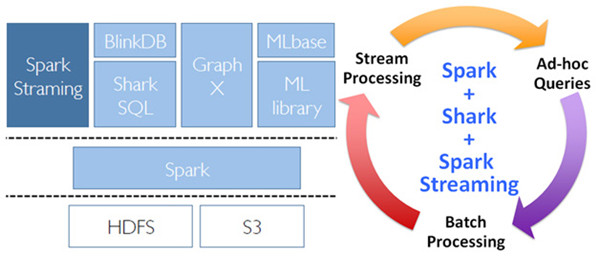
\includegraphics[width=6.5cm]{pic/spark_ecosystem.jpg} 
    \caption{Spark生态系统} \label{fig:spark_ecosystem} 
    \end{figure}
    Shark:Shark基本上就是在Spark的框架基础上提供和Hive一样的HiveQL命令接口,为了最大程度的保持和Hive的兼容性,Shark使用了Hive的API来实现query Parsing和 Logic Plan generation,最后的PhysicalPlan execution阶段用Spark代替HadoopMapReduce。通过配置Shark参数,Shark可以自动在内存中缓存特定的RDD,实现数据重用,进而加快特定数据集的检索。同时,Shark通过UDF用户自定义函数实现特定的数据分析学习算法,使得SQL数据查询和运算分析能结合在一起,最大化RDD的重复使用。
    SparkR:SparkR是一个为R提供了轻量级的Spark前端的R包。 SparkR提供了一个分布式的data frame数据结构,解决了 R中的data frame只能在单机中使用的瓶颈,它和R中的data frame 一样支持许多操作,比如select,filter,aggregate等等。(类似dplyr包中的功能)这很好的解决了R的大数据级瓶颈问题。 SparkR也支持分布式的机器学习算法,比如使用MLib机器学习库。SparkR为Spark引入了R语言社区的活力,吸引了大量的数据科学家开始在Spark平台上直接开始数据分析之旅。
  
%% 本章参考文献
\ifx\usechapbib\empty
\nocite{BSTcontrol}
\setcounter{NAT@ctr}{0}
\bibliographystyle{buptgraduatethesis}
\bibliography{bare_thesis}
\fi

